\documentclass[../Main.tex]{subfiles}

\begin{document}
\section{Definitions}
\begin{definition}{Modulo}
    Let $n \geq 2$. Then the integers \underline{modulo $n$}, $\Z_n$ or $\Z /n\Z$, consists of the integers with two integers regarded the same if they differ by a multiple of $n$.
\end{definition}
\begin{definition}{Congruence}
    Two integers are \underline{congruent} modulo $n$ if they differ by a multiple of $n$. We write
    \begin{equation*}
        \congruence{x}{y}{n}
    \end{equation*}
\end{definition}
We can view $\Z_n$ as a circle. For example, $Z_4$:
\begin{center}
    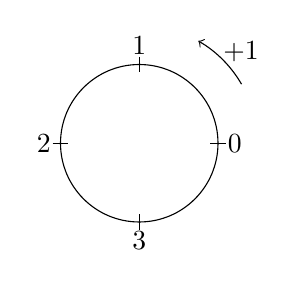
\begin{tikzpicture}
        \tikzset{
            smallline/.pic={
                \draw (0, 1mm) -- (0, -1mm);
            }
        }
        \draw (0, 0) pic[rotate=90] {smallline}
            node[anchor=west] {0}
            arc[radius=1, start angle=0, end angle=90]
            pic {smallline}
            node[anchor=south] {1}
            arc[radius=1, start angle=90, end angle=180]
            pic[rotate=90] {smallline}
            node[anchor=east] {2}
            arc[radius=1, start angle=180, end angle=270]
            pic {smallline}
            node[anchor=north]{3}
            arc[radius=1, start angle=270, end angle=360];

        \draw[->] (0.299, 0.75) arc[radius=1.5, start angle=30, end angle=60]
        node[pos=0.7, anchor=west] {$+1$};
    \end{tikzpicture}
\end{center}
\section{Arithmetic in \texorpdfstring{$\Z_n$}{Zn}}
\begin{propositions}[Arithmetic in $\Z_n$]{
        Let $\congruence{a}{a'}{n}$ and $\congruence{b}{b'}{n}$.
        \label{propArithmeticZn}
    }
    \item $\congruence{a + b}{a' + b'}{n}$ \label{propAdditionZn}
    \item $\congruence{a b}{a' b'}{n}$ \label{propMultZn}
\end{propositions}
\begin{proof}
    Note that we have $n | (a - a')$ and $n | (b - b')$
    \begin{enumerate}
        \item Addition mod $n$:
        We have $n | (a - a' + b - b')$. That is, $n | ((a+b) - (a' + b'))$. So $\congruence{a + b}{a' + b'}{n}$.
        \item Multiplication mod $n$:
        We have $n | (a - a')b$ and $n | (b - b')a'$, so combining these: $n | \left((a - a')b + (b - b')a'\right)$\par
        That is, $n | (ab - a'b')$, so $\congruence{ab}{a'b'}{n}$.
    \end{enumerate}
\end{proof}
So we have that congruences respect addition and multiplication, so we have all of the usual arithmetical operations (except division - see the next section).
\section{Solving Congruences}
We have the usual rules of arithmetic, so we consider what an \textit{equation} looks like in $\Z_n$. 
\begin{example}
    We consider the congruence:
    \begin{equation}
        \congruence{7x}{2}{10}
        \label{eqnSimpleCongruenceExample}
    \end{equation}
    We do not actually have a good idea of what division looks like yet, but we can use multiplication. Note that $\congruence{7 \times 3 = 21}{1}{10}$. Therefore, if we multiply equation~\ref{eqnSimpleCongruenceExample} by 3, we can remove the 7 multiplying $x$:
    \begin{align*}
        &\congruence{3 \times 7x}{3 \times 2}{10} \\
        &\congruence{x}{6}{10}
    \end{align*}
    And this is what a solution looks like in $\Z_n$ - the solutions are unique up to congruence.
\end{example}
\begin{definition}{Modular inverse}
    Given $a, b \in \Z_n$, we say that $b$ is an \underline{inverse} of $a$ if $\congruence{a \times b}{1}{n}$. If such a $b$ exists, we say that $a$ is \underline{invertible} or a \underline{unit} mod $n$. We write $a^{-1}$ for this inverse, if it exists.
\end{definition}
\begin{proposition}
    Inverses are unique modulo $n$.
\end{proposition}
\begin{proof}
    Suppose there exists integers $b$ and $b'$ such that $\congruence{ab}{1}{n}$ and $\congruence{ab'}{1}{n}$.\par
    \begin{align*}
        b &\equiv (ab')b \\
        &\equiv b'(ab) \\
        &\equiv b'
    \end{align*}
    So $\equiv{b}{b'}{n}$. That is, any two inverses must be congruent to each other.
\end{proof}
Now we have some form of division or cancellation in modulo arithmetic: if $a$ is a unit, then we can say $\congruence{ab}{ac}{n} \implies \congruence{b}{c}{n}$.
\begin{proposition}
    Let $n \geq 2$. $a$ is a unit mod $n$ if and only if $a$ and $n$ are coprime.
    \label{propUnitsCoprimes}
\end{proposition}
\begin{proof}
    We have $\hcf{(a, n)} = 1$, so by theorem~\ref{thmLinearComboHCF}, we have some integers $x$ and $y$ such that $ax + ny = 1$.\par
    This is equivalent to $ax = 1 - ny$, or $\congruence{ax}{1}{n}$, and we note that $x$ is the inverse of $a$.
\end{proof}
\begin{corollary}
    For $a$ and $n$ coprime, the congruence $\congruence{ax}{b}{n}$ has a unique solution.
    \label{corCongruenceSolutions}
\end{corollary}
We end up with a similar result to \ref{thmBezout} for congruences of the form
\begin{equation}
    \congruence{ax}{b}{n}, \text{ where } \hcf{(a, n)} = d > 1
    \label{eqnHCFCongruence}
\end{equation}
We then find that there is a solution if and only if $d | b$. In this case, dividing equation~\ref{eqnHCFCongruence} by $d$ gives an equation of the form discussed in corollary~\ref{corCongruenceSolutions}.
\section{Simulataneous congruences}
In order to solve simultaneous congruences, we need an important theorem.
\begin{theorem}[Chinese Remainder Theorem]
    Let $m$ and $n$ be coprime. Let $a, b \in \Z$.\par
    Then there is a unique solution to the simultaneous congruences:
    \begin{align*}
        &\congruence{x}{a}{m} \\
        &\congruence{x}{b}{n} \\
    \end{align*}
    that is unique modulo $mn$.
    \label{thmChineseRemainder}
\end{theorem}
\begin{proof}
    We first find a solution.\par
    Since $m$ and $n$ are coprime, we have $s m + t n = 1$ for some integers $s$ and $t$. Therefore, $\congruence{sm}{1}{m}$ and $\congruence{tn}{1}{m}$.\par
    Now consider the linear combination $x = a(tn) + b(sm)$. Then we have:
    \begin{align*}
        &\congruence{x}{a + 0}{m} \\
        &\congruence{x}{b + 0}{n} 
    \end{align*}
    So $x$ solves the simultaneous congruences.\par
    We then show this solution is unique.\par
    Suppose $y$ is also a solution, so $\congruence{y}{a \equiv x}{m}$ and $\congruence{y}{b \equiv x}{m}$.\par
    Then:
    \begin{align*}
        &\implies m | (y - x) \text{ and } n | (y - x) \\
        &\implies mn | (y - x) \text{ since } \hcf{(m, n)} = 1 \\
        &\implies \congruence{y}{x}{mn}
    \end{align*}
\end{proof}
\begin{remark}
    Theorem~\ref{thmChineseRemainder} can also be extended by induction to systems of more than 2 simultaneous congruences.
\end{remark}
\section{More on Exponentiation in \texorpdfstring{$\Z_n$}{Zn}}
We first introduce a very interesting function that can simplify theorems relating to exponentiation in $\Z_n$.
\begin{definition}{Euler totient function}
    For a natural number $n$, denote the number of integers $a$ with $1 \leq a \leq n$ that are coprime with $n$ as $\varphi(n)$. The function $\varphi$ is the \underline{Euler totient function}.
\end{definition}
Note that $\varphi(1)$ is 1.\par
If $p$ is a prime, $\varphi(p) = p - 1$. If, further, $q$ is a prime, then $\varphi(pq) = pq - p - q + 1$.
\begin{example}
    What are the powers of 2 mod 7?\par
    \begin{equation*}
        2^1 \equiv 2, 2^2 \equiv 4, 2^3 \equiv 1, 2^4 \equiv 2, \cdots
    \end{equation*}
\end{example}
We can introduce some theorems to make this process easier.
\begin{theorem}[Fermat's Little Theorem]
    Let $p$ be prime. Then $\congruence{a^p}{a}{p}$.
    \label{thmFermatLittle}
\end{theorem}
The theorem is alternately stated $\congruence{a^{p-1}}{1}{p}$ if $a \neq 0$.
\begin{proof}
    If $a = 0$ then we are done.\par
    If $a \neq 0$ then $a$ is a unit mod $p$ by proposition~\ref{propUnitsCoprimes}. Therefore, $\congruence{ax}{ay}{p}$ if and only if $\congruence{x}{y}{p}$. Hence the numbers
    \begin{equation*}
        a, 2a, \cdots, (p-1)a
    \end{equation*}
    are pairwise incongruent and non-zero. Therefore, they must be some permutation of $\{1, 2, \cdots, p-1\}$. Then consider their product:
    \begin{align*}
        (a)(2a)\cdots((p-1)a) &\equiv (1)(2)\cdots(p-1)\text{ mod } p \\
        a^{p-1}(p-1)! &\equiv (p-1)! \\
        a^{p-1} &\equiv 1 \text{ since all integers are units.}
    \end{align*}
\end{proof}
We can also extend this to non-prime elements by requiring coprimality.
\begin{theorem}[Euler-Fermat Theorem]
    \label{thmEulerFermat}
    Let $a$ and $m$ be coprime integers. Then $\congruence{a^{\varphi(m)}}{1}{m}$.
\end{theorem}
\begin{proof}
    Let $U$ be the set of units:
    \begin{equation*}
        U = \subsetselect{x \in \Z}{0 < x < m, \hcf{(x, m)} = 1}
    \end{equation*}
    And label each element $u_1, \cdots, u_{\varphi(m)}$.\par
    Then $a u_1, a u_2, \cdots, a u_{\varphi(m)}$ are all distinct and invertible mod $m$ since $a$ is a unit (by assumption). They are thus congruent to the elements of $U$ after permutation. Consider their product:
    \begin{align*}
        \prod_{u \in U} a u &\equiv \prod_{u \in U} u \\
        a^{\varphi(m)} \prod_{u \in U} u &\equiv \prod_{u \in U} u
    \end{align*}
    But a product of units is invertible:
    \begin{equation*}
        \congruence{a^{\varphi(m)}}{1}{m}
    \end{equation*}
\end{proof}
\section{Asymmetric Encryption}
\end{document}